\documentclass{article}
\usepackage[utf8]{inputenc}
\usepackage[english]{babel}
\usepackage{amsthm}
\usepackage{amsmath}
\usepackage{amssymb}
\usepackage{mathtools}
\usepackage{mathrsfs}
\usepackage{enumerate}
\usepackage{chngcntr}
\usepackage{sectsty}
\usepackage{xfrac}
\usepackage{bbm}
\usepackage{hyperref} % Uncommment to make references clickable
\usepackage[a4paper,margin=1.3in,footskip=0.25in]{geometry}

% Creating command `renewtheorem'. Used in the section `main results' to temporarily change the numbering of theorems so that we can have `theorem 1' and not `theorem 2.1'. 
\makeatletter
\def\renewtheorem#1{%
  \expandafter\let\csname#1\endcsname\relax
  \expandafter\let\csname c@#1\endcsname\relax
  \gdef\renewtheorem@envname{#1}
  \renewtheorem@secpar
}
\def\renewtheorem@secpar{\@ifnextchar[{\renewtheorem@numberedlike}{\renewtheorem@nonumberedlike}}
\def\renewtheorem@numberedlike[#1]#2{\newtheorem{\renewtheorem@envname}[#1]{#2}}
\def\renewtheorem@nonumberedlike#1{  
\def\renewtheorem@caption{#1}
\edef\renewtheorem@nowithin{\noexpand\newtheorem{\renewtheorem@envname}{\renewtheorem@caption}}
\renewtheorem@thirdpar
}
\def\renewtheorem@thirdpar{\@ifnextchar[{\renewtheorem@within}{\renewtheorem@nowithin}}
\def\renewtheorem@within[#1]{\renewtheorem@nowithin[#1]}
\makeatother

% Configuring style of references
\hypersetup{
    colorlinks = True,
    allcolors = blue	
}

% Makes equation numbering based on section
\counterwithin{equation}{section}

% Changing the styling of section and subsection titles. Comment to get default styling
\sectionfont{\centering\mdseries\scshape}
\subsectionfont{\mdseries\scshape}

%%%%%%%%%%%%%%%%%%%%%%%%%%% Defining environments %%%%%%%%%%%%%%%%%%%%%%%%%%%%%%%%%%%%%%%%
\newtheoremstyle{slimDefinitionStyle} % name
    {\topsep}                    	  % Space above
    {\topsep}                    	  % Space below
    {}			                   	  % Body font
    {}                           	  % Indent amount
    {\mdseries\scshape}			  	  % Theorem head font
    { ---}                            % Punctuation after theorem head
    {.5em}                       	  % Space after theorem head
    {}  % Theorem head spec (can be left empty, meaning ‘normal’)
\newtheoremstyle{slimTheoremStyle} 	% name
    {\topsep}                    	% Space above
    {\topsep}                    	% Space below
    {\itshape}                   	% Body font
    {}                           	% Indent amount
    {\mdseries\scshape}			 	% Theorem head font
    { ---}                          % Punctuation after theorem head
    {.5em}                       	% Space after theorem head
    {}  % Theorem head spec (can be left empty, meaning ‘normal’)
\theoremstyle{slimTheoremStyle} % Comment this to get boldface theorem headers

\newtheorem{theorem}{Theorem}[section]
\newtheorem{corollary}{Corollary}[theorem]
\newtheorem{lemma}[theorem]{Lemma}
\newtheorem{proposition}[theorem]{Proposition}

% \theoremstyle{definition}
\theoremstyle{slimDefinitionStyle}
\newtheorem{definition}{Definition}[section]

\theoremstyle{remark}
\newtheorem{remark}{Remark}[section]
\newtheorem{notation}{Notation}[section]

%%%%%%%%%%%%%%%%%%%%%%%%%% Defining custom commands %%%%%%%%%%%%%%%%%%%%%%%%%%%%%%%%%%%%%%%
% Common fonts
\renewcommand{\cal}[1]{\mathcal{#1}}
\newcommand{\scr}[1]{\mathscr{#1}}
\newcommand{\bb}[1]{\mathbb{#1}}

% Common sets
\newcommand{\R}{\mathbb{R}}
\newcommand{\N}{\mathbb{N}}
\newcommand{\Z}{\mathbb{Z}}

% Expectation
\newcommand{\E}{\mathbb{E}}
\newcommand{\Ex}[1]{\mathbb{E}\left[ #1 \right]}
\newcommand{\ExCond}[2]{\mathbb{E} \left[\left. #1 \right| #2 \right]}

% Probability
\renewcommand{\P}{\mathbb{P}}
\renewcommand{\Pr}[1]{\mathbb{P} \left( #1 \right)}
\newcommand{\PrCond}[2]{\mathbb{P} \left( \left. #1 \right| #2 \right)}

% Common distributions 
\newcommand{\dNorm}[2]{\mathcal(N)\left( #1, #2 \right)}
\newcommand{\dExp}[1]{\text{Exp} \left( #1 \right)}
\newcommand{\dBer}[1]{\text{Ber} \left( #1 \right)}
\newcommand{\dPoi}[1]{\text{Po} \left( #1 \right)}

% Miscellaneous math stuff
\newcommand{\defeq}{\vcentcolon=}
\newcommand{\eqdef}{=\vcentcolon}
\DeclarePairedDelimiter\ceil{\lceil}{\rceil}
\DeclarePairedDelimiter\floor{\lfloor}{\rfloor}

%%%%%%%%%%%%%%%%%%%%%%%%%%%%%%%%%%%%%%%%%%%%%%%%%%%%%%%%%%%%%%%%%%%%%%%%%%%%%%%%%%%%%%%%%%%


\begin{document}

\section{Introduction and construction}\label{dec:introduction}

\begin{quote}
{\small We introduce the main objects of study and briefly describe the construction of the corresponding stochastic processes. The construction gives rise to important properties that we discuss. }
\end{quote}

\subsection{Introduction}\label{ssec:introduction}
The East process is an interacting particle system evolving with a Glauber like dynamics on the state space $\Omega \defeq \{0,1\}^\Z$. It belongs to a class of stochastic processes called kinetically constrained spin models (KCMs), with the East process being the first of these to be studied rigorously. The process evolves as follows: at each site $x \in \Z$ the system tries to update the value of the spin at $x$ to 1 or 0 at rate $p \in (0,1)$ and $q \defeq 1 - p$ respectively. The update is accepted only if a local constraint is satisfied, which in the East process's case is that the occupation variable at site $x-1$ must be equal to 1. Sometimes we will call elements of $\Omega$ \textit{configurations} and say a site is \textit{occupied} or \textit{infected} if its spin value is equal to 1. \\

In the sections to follow we focus on two objects of interest related to the East process. The first one is the speed of the so-called \textit{front}. Consider an East process started from the configuration equal to all 0 except at the origin. It is easy to see that the spins on $(-\infty, 0]$ stay frozen for all time, and infection 'spreads' to the right. A natural question to ask then is how fast this spreading of infection happens \textit{if} it happens at all. We define the front to be the rightmost infected site in the configuration at time $t$. In our study of the speed of the front we will compare the East process to a second stochastic process called the one-sided contact process. The one-sided contact process has the same state space $\Omega$ and evolves as follows: each site \textit{recovers} i.e. sets its spin to 0 at rate $q$ and gets infected by its left neighbour (provided the neighbour is infected) at rate $p$. The second object of interest is the \textit{mixing time} of the East process when restricted to $\{ 0, 1, ..., L\}$ for some $L \in \N^+$. We will study the mixing time for the East process on $\{ 0, 1, ..., L\}$ with the occupation variable of the origin fixed to be $1$, so that the evolution at site 1 is unconstrained. \\

The main results of this paper can be summarised as follows. We show that for $p$ larger than a critical value the front of the East process started from exactly one infection propagates at precisely linear speed. We also show that for such $p$ the mixing time on $\{ 0, 1, ..., L\}$ is $\Theta(L)$\footnote{We say $f = \Theta(g)$ if there exist constants $K_1, K_2$ such that for all large enough $n \in \N$ it holds that $K_1 g(n) \leq f(n) \leq K_2 g(n)$.}. In the process of proving these we show exponential bounds on the front propagation and survival time of the one-sided contact process. The results concerning the East process have been known to hold under weaker restrictions on $p$ for some time, see \cite{ganguly2015cutoff} for a review. The results concerning the one-sided contact process were first stated in \cite{durrett1983supercritical}, but to our knowledge never proved in detail. The paper is broken into 5 chapters. The second chapter contains the statements of our main results. Chapter three discusses the one-sided contact process and presents proofs of the above mentioned exponential bounds. Chapter four is devoted to the proof of Theorem \ref{main_thm:speed} while in chapter five we present the proof of Theorem \ref{main_thm:mixing}. 


\subsection{Constructing the basic coupling}
Let $\scr{C} = (E_{x,k}, B_{x,k})_{x \in \Z, k \in \N^+}$ be a collection of independent random variables with $E_{x,k} \sim \dExp{1}$ and $B_{x,k} \sim \dBer{p=1-q}$. Define the times 
\[
T_{x,n} \defeq \sum\limits_{k=1}^n E_{x,k}
\]
 also referred to as \textit{clock rings} and call a clock ring $T_{x,n}$ \textit{legal} if the local constraint of the corresponding process is satisified at site $x$ at time $T_{x,n}$. We can now construct the East process $(\sigma_t)_{t \geq 0}$ and the one-sided contact process $(\eta_t)_{t \geq 0}$ using $\scr{C}$ as follows. 
 
For each site $x \in \Z$ at each time $T_{x,n}$:
\begin{itemize}
  \item If $B_{x,n} = 1$:
  \begin{enumerate}
  	\item If $\sigma_{T^-_{x,n}} (x-1) = 1$ update $\sigma$ to 1 at site $x$. 
  	\item If $\eta_{T^-_{x,n}} (x-1) = 1$ update $\eta$ to 1 at site $x$. 
  \end{enumerate}
  \item Else:
  \begin{enumerate}
  	\item If $\sigma_{T^-_{x,n}} (x-1) = 1$ update $\sigma$ to 0 at site $x$. 
  	\item Update $\eta$ to 0 at site $x$. 
  \end{enumerate}
\end{itemize}

\begin{figure}[!h]
  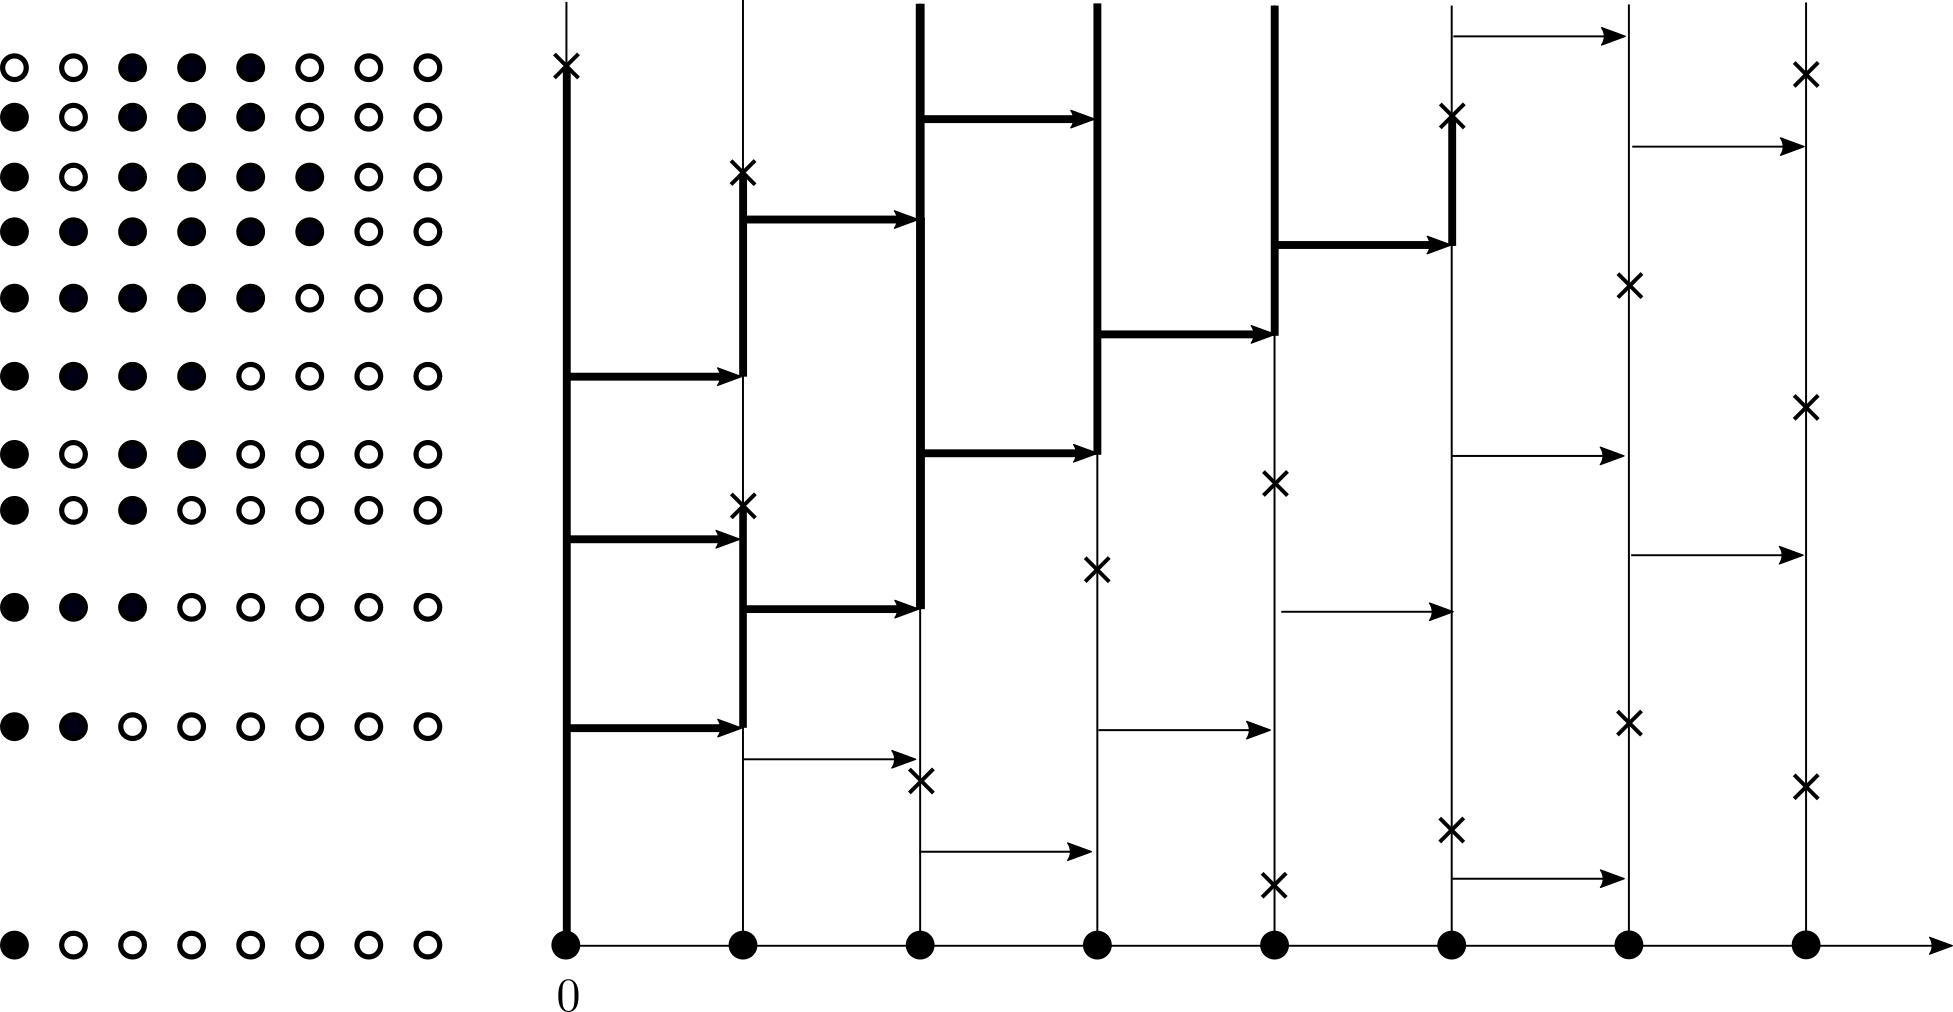
\includegraphics[width=\linewidth]{images/graphical_construction}
  \caption{Harris' graphical representation, showing the evolution of a one-sided contact process started from site $0$. }
  \label{fig:graphical_construction}
\end{figure}

There is a graphical representation of $\scr{C}$ introduced by Harris that is a helpful tool for visualizing the evolution of the two coupled processes however we will only use it to analyze the one-sided contact process. We will use the symbol $\scr{P}$ to refer to this graphical construction which we informally describe as follows. First draw vertical lines from $0$ to infinity at each integer in $\Z$. At each site $x \in \Z$ put a cross on the line at $(x, T_{x,n})$ if $B_{x,n} = 0$. If $B_{x,n} = 1$ instead of a cross draw an arrow from $(x - 1, T_{x,n})$ to $(x, T_{x,n})$. Crosses represent recovery while arrows represent infection spreading towards the right. For an example of the graphical representation see Figure \ref{fig:graphical_construction}. 

\begin{notation}[Initial configurations]
Suppose we start a stochastic process $(\xi_t)_{t \geq 0}$ with state space $\Omega$ from initial configuration $\zeta \in \Omega$. The resulting process will be denoted $(\xi^\zeta_t)_{t \geq 0}$. If $\nu$ is a probability distribution on $\Omega$, then we write $(\xi^\nu_t)_{t \geq 0}$ for the process started from a \textit{random} distribution drawn from $\nu$. The initial distribution is drawn independently from $\scr{C}$
\end{notation}
\begin{notation}[$\Omega$ and $\cal{P}(\Z)$]\label{not:powerset}
Because of the natural bijection between the power set of $\Z$ and $\Omega$, we will consider configurations as both subsets of $\Z$ and elements of $\Omega$, regularly switching between the two interpretations. 
\end{notation}

In what follows we only consider contact processes with $p > p_c$ where $p_c$ is the critical parameter for the one-sided contact process, defined as $p_c \defeq \sup\{ p : |\eta^{\{0\}}_t| \rightarrow 0\ a.s.\}$. A one-sided contact process with rates satisfying this condition is called supercritical. By definition the extinction time $\tau(\eta^{\{0\}}_.) \defeq \inf\{t \geq 0 \mid \eta^{\{0\}}_t = \varnothing \}$ of a supercritical one-sided contact process satisfies $\Pr{\tau(\eta^{\{0\}}_.) = \infty} > 0$ i.e. the process survives forever with positive probability. 

\begin{notation}[Supercritical East process]
As per the previous discussion, we call an East process supercritical if $p > p_c$. 
\end{notation}

\subsection{Domination and other properties}\label{ssec:intro_properties}
The basic coupling has two important properties that follow immediately from its definition. First, it lets us construct both processes started from any initial configuration on the same probability space. The second property is domination: if at some time $t \geq 0$ it holds that $\eta_t \leq \sigma_t$ then $\eta_{t+s} \leq \sigma_{t+s},\ \forall s \geq 0$. To see this note that under the graphical construction $\eta$ updates a particular site to 1 only if $\sigma$ does too, and $\sigma$ updates a particular site to 0 only if $\eta$ does too. In particular, if $X(\cdot)$ denotes the position of the front then $X(\eta_{t+s}) \leq X(\sigma_{t+s}),\ \forall s \geq 0$. \\

Domination is what enables us to bound the East process from below by the one-sided contact process. The reason we might want to do this is that contact processes posess desirable qualities that KCMs in general might not. Contact processes are \textit{attractive} in the sense that if $\nu \subseteq \xi \subseteq \Z$ then $\eta^\nu_t \leq \eta^\xi_t$ for all $t \geq 0$ under the basic coupling. Moreover they are also \textit{additive}: if $\nu, \xi \subseteq \Z$ then $\eta^{\nu \cup \xi}_t = \eta^\nu_t \cup \eta^\xi_t$ for all $t \geq 0$ under the basic coupling. These qualities make contact processes more amenable to analysis than KCMs, and there is a breadth of methods and results already established. The East process lacks both attractivity and additivity, thus the desire to compare it to the `simpler' one-sided contact process is justified. 


\theoremstyle{slimTheoremStyle}
\renewtheorem{theorem}{Theorem}

\section{Main results}\label{sec:results}

To state our first result we need to define the \textit{front}. Recall the notation used in Subsection \ref{ssec:intro_properties} to denote the rightmost site of a configuration in $\Omega$. Keeping in mind the identification of $\Omega$ and $\cal{P}(\Z)$ described in Notation \ref{not:powerset} we define
\begin{definition}
For $A \subseteq \Z$ we write $X(A) \defeq \max (A) \in \N \cup \{-\infty, \infty \}$ with $\max(\varnothing) \defeq -\infty$ for the \textit{front} of $A$. 
\end{definition} 

\begin{theorem}\label{main_thm:exponential_bounds}
If $(\eta_t)_{t \geq 0}$ is a supercritical, one-sided contact process then there exists $\alpha > 0$ such that for all $a < \alpha$ there exist constants $\gamma, C > 0$ such that for all $t \geq 0$ we have
\begin{align*}
  \Pr{X(\eta^{(-\infty, 0]}_t) < a t} &\leq C e^{-\gamma t}. 
  \intertext{Furthermore there exist constants $\gamma, C > 0$ such that for all $t \geq 0$ it holds that}
  \Pr{t < \tau(\eta^{\{0\}}_.) < \infty } &\leq C e^{-\gamma t}.  
\end{align*}
\end{theorem}

Using these results for the supercritical one-sided contact process we go on to show 

\begin{theorem}\label{main_thm:speed}
Let $(\sigma^{\{0\}}_t)_{t \geq 0}$ be an East model. Then there exist constants $v, \gamma > 0$ such that for all $t \geq 0$ we have
\begin{align*}
\Pr{X(\sigma^{\{0\}}_t) > vt} &\leq e^{- \gamma t}. \\
\intertext{Furthermore, if $(\sigma^{\{0\}}_t)_{t \geq 0}$ is supercritical then $\exists\ \alpha > 0$ such that $\forall\ a < \alpha$ there exist constants $\gamma, C > 0$ such that for all $t \geq 0$ it holds that } 
\Pr{X(\sigma_t) < at} &\leq C e^{-\gamma t}.
\end{align*}
\end{theorem}

Our third result concerns the \textit{mixing time} of the East model. To make sense of this first we need the notion of \textit{total variation distance} and \textit{distance from equilibrium}. 
\begin{definition}[Total variation distance]
Let $(\Omega, \cal{F})$ be a measurable space and $\nu, \mu$ be two probability measures on it. The total variation distance of $\nu$ and $\mu$ is defined as $\left\Vert \nu(\cdot) - \mu(\cdot) \right\Vert_{TV} \defeq \sup\limits_{A \in \cal{F}} \left| \nu(A) - \mu(A) \right|$
\end{definition}
\begin{definition}[Distance from equilibrium]\label{def:eq_distance}
Let $N \defeq (N_t)_{t \geq 0}$ be a continuous time, irreducible Markov chain taking values in a finite state space $\Omega$ and let $\pi$ be its equilibrium distribution. For $t \geq 0$ define 
\begin{equation}\nonumber
d(t) \defeq \max\limits_{x \in \Omega} \left\Vert \PrCond{N_t \in \cdot\ }{N_0 = x} - \pi(\cdot) \right\Vert_{TV} 
\end{equation}
to be the worst case total variation distance from equilibrium. 
\end{definition}

When restricted to $\{0, 1, ... L\}$, the East model with a fixed 1 at the origin is a finite, irreducible, continuous time Markov chain with equilibrium measure $\pi_L \defeq \delta_{1} \times \dBer{p}^L$. The mixing time then can be described as the time it takes to get close to the equilibrium distribution:
\begin{definition}[Mixing time of East model]
The mixing time of the East model with a fixed 1 at the origin is defined as $T^L_{mix} \defeq \inf\left\{ t \geq 0 \mid d(t) \leq \sfrac{1}{4} \right\}$. 
\end{definition}

\begin{theorem}\label{main_thm:mixing}
For every East model there exists a constant $K > 0$ such that $T^L_{mix} \leq KL$ for all $L \in \N$. Moreover, if the East model is supercritical then there exists a constant $K' > 0$ such that $K'L \leq T^L_{mix}$ for all $L \in \N$. 
\end{theorem}

\renewtheorem{theorem}{Theorem}[section]


\section{The one-sided contact process --- Proof of Theorem $1$}
\label{sec:contact}

\begin{quote}
{\small We review some results about the one-sided contact process and construct a link to a one-dependent oriented percolation model. We then exploit this link to obtain exponential bounds on the front propagation and survival times of the one-sided contact process. }
\end{quote}

\subsection{Classic results}

\begin{theorem}[{{\cite[Section 2.2]{liggett1977stochastic}}} and {{\cite[page 898, Claim III]{durrett1983supercritical}}}]\label{thm:upper_invariant}
If $(\eta_t)_{t \geq 0}$ is a one-sided contact process then $\Pr{\eta^\Z_t \in \cdot} \rightharpoonup \Pr{\eta^\Z_\infty \in \cdot} \eqdef \nu(\cdot)$ as $t \to \infty$ where $\nu$ is stationary, furthermore $\{ \eta^\Z_\infty (x) \}_{x \in \Z}$ is a stationary (shift) ergodic sequence. 
\end{theorem}

\begin{definition}
We call a one-sided contact process \textit{ergodic} if $\nu = \delta_{\{0\}}$ and \textit{nonergodic} otherwise. 
\end{definition}

\begin{remark}\label{rem:positive_density}
$\nu$ is sometimes called the \textit{upper invariant measure}. It is clear that $\nu$ is translation invariant, thus if we define $\rho \defeq \Pr{\nu(0) = 1}$ to be the probability that a given site is occupied under $\nu$, it follows that $\eta$ is ergodic if and only if $\rho = 0$. 
\end{remark}

\begin{lemma}\label{lem:old_results}
Let $\eta \defeq (\eta_t)_{t \geq 0}$ be a supercritical one-sided contact process. Then: 
\begin{enumerate}[(i)]
	\item $\eta$ is nonergodic
	\item For any $\Z \supseteq A \neq \varnothing$ it holds that $\Pr{\tau(\eta^A_t) = \infty} > 0$
	\item $\lim\limits_{M \rightarrow \infty} \sup\limits_{A \subseteq \Z: |A| = M} \Pr{\tau(\eta^A_t) = \infty} = 1$
	\item $\eta^\Z_t \geq \nu$ for all $t \geq 0$
	\item For all $\epsilon > 0$ and $M \in \N$, if $N$ is large enough then it holds that 
		\[\nu([0, N] \cap \cdot\text{ contains an interval of length $M$ }) > 1 - \epsilon. \]  
\end{enumerate}
\end{lemma}

\begin{proof}
The proof of (i) is given at \cite[page 902, top]{durrett1980growth}. For (ii) see \cite[Theorem 9.1]{harris1974contact} while (iii) can found in \cite[Lemma 5.2]{griffeath1979additive}. \\ 

To prove $(iv)$ consider the one-sided contact process $(\eta^\nu_t)_{t \geq 0}$ started from initial distribution $\nu$ constructed using $\scr{P}$. Note that since $\nu$ is stationary, $\eta^\nu_t \sim \nu$ for all $t \geq 0$. To conclude note that $\eta^\nu_0 \leq \eta^\Z_0 = \Z$ almost surely so that by attractivity $\eta^\nu_t \leq \eta^\Z_t$ for all $t \geq 0$ almost surely. \\

To prove $(v)$, let $\theta : \Omega \rightarrow \Omega$ be the left shift operator given by $\theta(\xi)(x) \defeq \xi(x + 1)$ and define $f : \Omega \rightarrow \{0, 1\}$ as $f(\xi) \defeq \mathbbm{1}_{\{\xi(1) = \xi(2) = ... = \xi(M) = 1\}}$. By Theorem \ref{thm:upper_invariant} $\theta$ is ergodic with respect to $\nu$ so that by Birkhoff's ergodic theorem it holds that 
\begin{equation} \label{eqn:birkhoff}
\frac{1}{N} \sum\limits^{N - 1}_{n = 0} f(\theta^n \eta^\Z_\infty) \xrightarrow[a.s.]{N \rightarrow \infty} \Ex{f(\eta^\Z_\infty)} = \nu(\, \cdot\, \supset \{1, ..., M\} ). 
\end{equation}
Once again consider the supercritical one-sided contact process $(\eta^\nu_t)_{t \geq 0}$ started from initial distribution $\nu$. By stationarity it follows that
\begin{align*}
\nu(\, \cdot\, \supset \{1, ..., M\}) &= \Pr{\eta^\nu_t \supset \{1, ..., M\}}                                    && \forall\, t \geq 0 \\
									  &\geq \Pr{\eta^\nu_0 (0) = 1 \text{ and } \eta^\nu_t \supset \{1, ..., M\}} && \forall\, t \geq 0. 
\end{align*}

Define $G(M, t)$ to be the event that in the time interval $[0, t]$ there are exactly $M$ clockrings when restricted to sites in $[0, M]$ and they satisfy $0 \leq T_{1, 1} < T_{2, 1} < ... < T_{M, 1} \leq t$. By basic properties of the exponential distribution for $t > 0$ we have
\begin{equation}\nonumber
\Pr{G(M, t)} > 0. 
\end{equation}
With this we can show that $\Ex{f(\eta^\Z_\infty)} > 0$: 
\begin{align*}
\Pr{\eta^\nu_0 (0) = 1 \text{ and } \eta^\nu_t \supset \{1, ..., M\}} &\geq \PrCond{\eta^\nu_t \supset \{1, ..., M\}}{\{\eta^\nu_0 (0) = 1\} \cap G(M, t)} \\ 
&\qquad \times \Pr{\eta^\nu_0 (0) = 1} \Pr{G(M, t)} \\
&\geq p^M \Pr{\eta^\nu_0 (0) = 1} \Pr{G(M, t)}. 
\end{align*}
Since $(\eta^\nu_t)_{t \geq 0}$ is supercritical $\rho = \Pr{\eta^\nu_0 (0) = 1} > 0$ by part (i) and Remark \ref{rem:positive_density}. By (\ref{eqn:birkhoff}) it follows that $\eta^\Z_\infty$ contains an interval of length $M$ almost surely infinitely many times. Thus we can choose $N$ large enough such that $\eta^\Z_\infty \cap [-N, N]$ contains an interval of length $M$ with probability greater than $1 - \epsilon$. By translation invariance the same holds for $\eta^\Z_\infty \cap [0, 2N]$ and the result follows. 
\end{proof}

\begin{definition}
Let $\eta \defeq (\eta_t)_{t \geq 0}$ be a one-sided contact process. For $A \subseteq \Z$ define $r^A_t \defeq \sup\eta^A_t$ and $l^A_t \defeq \inf\eta^A_t$ to be the right and left edge processes of $(\eta^A_t)_{t \geq 0}$. 
\end{definition}
\begin{remark}
Note that by definition $r^A_t = X(\eta^A_t)$ however the former notation is more convenient for what follows. 
\end{remark}

\begin{theorem}[{{\cite[page 6 (c)]{durrett1983supercritical}}}]\label{thm:convergence}
Let $(\eta_t)_{t \geq 0}$ be a supercritical one-sided contact process. Then there exist constants $0 \leq \beta < \alpha$ such that for all $|A| < \infty$, on $\{\tau(\eta^A_\cdot) = \infty\}$ it holds that
\begin{equation}\nonumber
\frac{r^A_t}{t} \xrightarrow[a.s.]{t \rightarrow \infty} \alpha \hspace{5mm} \text{and} \hspace{5mm} \frac{l^A_t}{t} \xrightarrow[a.s.]{t \rightarrow \infty} \beta.
\end{equation}
\end{theorem}

\subsection{Percolation construction}

\begin{figure}[!h]
  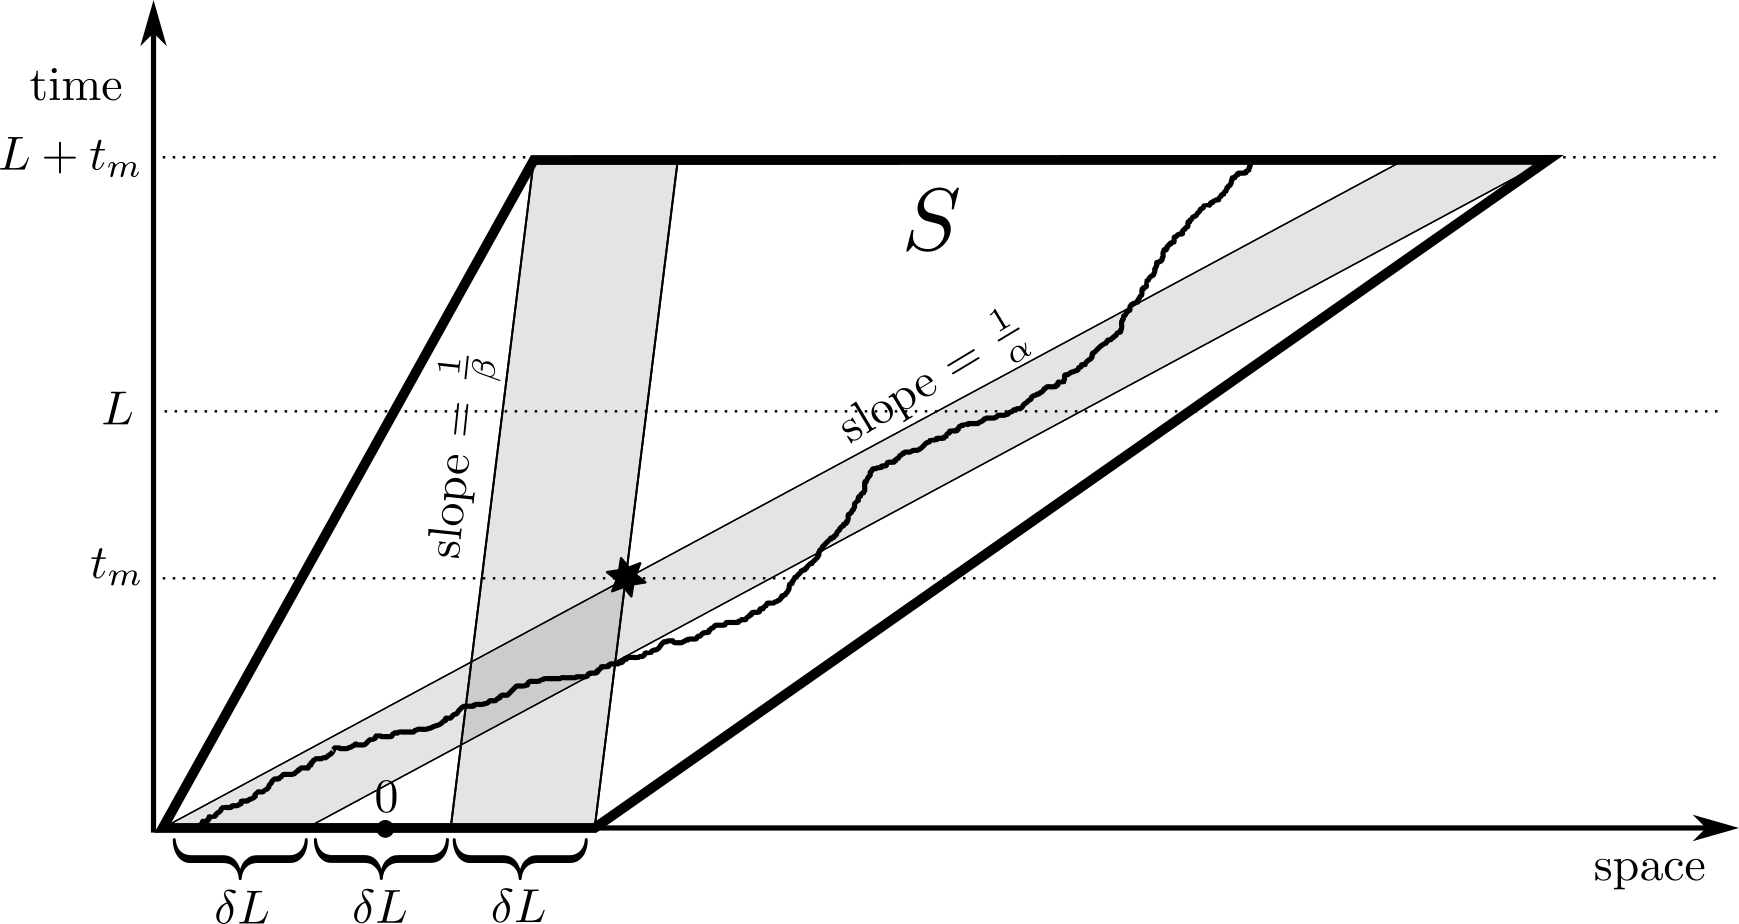
\includegraphics[width=\linewidth]{images/construction_single_tile}
  \caption{A visualisation of $S$ and a right nice path. }
  \label{fig:construction_single_tile}
\end{figure}

\begin{definition}
A \textit{path} in the graphical representation $\scr{P}$ connecting space-time points $(x, t), (y, s)$ with $t \leq s$ is a set of points $\{(z(r), r) \in \Z \times \Z_{\geq 0} \}_{r \in [t,s]}$ parametrised by $r \in [t, s]$ such that 
\begin{enumerate}[(i)] 
\item $z(t) = x$ and $z(s) = y$
\item No recovery occurs in $\{(z(r), r)\}_{r \in [t,s]} \subset \scr{P}$
\item The trajectory follows arrows i.e. $z(r-) \neq z(r)$ only if there is an arrow from $z(r-)$ to $z(r)$ at time $r$.   
\end{enumerate}
\end{definition}

Let $\delta > 0$ be a constant and $S$ be the convex quadrilateral defined by the four vertices $\{(- \frac{3 \delta L}{2}, 0), (\frac{3 \delta L}{2}, 0), (\beta (L + t_m) + \frac{3 \delta L}{2}, L + t_m), (\alpha (L + t_M) - \frac{3 \delta L}{2}, L + t_m) \}$, see Figure \ref{fig:construction_single_tile} for reference. Let $t_m = \frac{3\delta L }{\alpha - \beta}$ and define R to be the event that a \textit{right nice path} exists, which is a path inside $S$ that starts from $(- \frac{3 \delta L}{2}, - \delta L) \times \{0\}$ goes through $(\alpha t_m - \frac{ 3 \delta L }{2}, \infty) \times \{t_m\}$ and through $(\alpha L - \frac{3 \delta L}{2},\alpha L - \frac{\delta L}{2}) \times \{L\}$ and reaches $\Z \times \{ L + t_m \}$. In other words, looking at Figure \ref{fig:construction_single_tile}, a path inside $S$ that starts from $(- \frac{3 \delta L}{2}, - \delta L) \times \{0\}$, falls to the right of the star at time $t_m$, falls inside the right gray-shaded region at time $L$ and survives until time $L + t_m$. The star lies at the last intersection of the two shaded areas, which is easily checked to occur at time $t_m$. We always take $\delta < \frac{(\alpha - \beta)}{3}$ so that $t_m < L$. Analogously, for the left side define \textit{left nice paths} and the event $H$ that one occurs. Finally, let $E \defeq R \cap H$ be the event that both left and right nice paths exist. \\

\begin{lemma}\label{lem:construction}
For fixed $\frac{\alpha - \beta}{3} > \delta$ and $\epsilon > 0$ we can take $L$ large enough such that $R$ happens with probability greater than $1 - \epsilon$.  
\end{lemma}

\begin{remark}
From here on in this section `with high probability' is equivalent to `with probability greater than $1 - k \epsilon$' for some integer $k$ independent of $\epsilon$. We will sometimes abbreviate `with high probability' to `w.h.p.'.  
\end{remark}

\begin{proof}
Let $I_\delta = \left( \frac{ - 3 \delta L}{2}, - \delta L \right)$. By Lemma \ref{lem:old_results} part $(iii)$ we may take $L$ large enough so that $(\eta^{I_\delta}_t)_{t \geq 0}$ survives with high probability - call this threshold $L'$. As a consequence of almost sure convergence of the velocity of the edge processes, we can take $L$ large enough such that $(r^{I_\delta}_t)_{t \geq 0}$ goes through $(\alpha t_m  - \frac{5 \delta L }{4}, \infty) \times \{t_m\}$ and through $(\alpha L - \frac{5 \delta L}{4}, \alpha L + \frac{\delta L}{2}) \times \{L\}$ with high probability. Similarly for the left edge process, for large enough $L$ we have $l^{- I_\delta}_{t_m} < \alpha t_m - \frac{3 \delta L}{2}$ w.h.p. so that $l^{- I_\delta}_t$ and $r^{I_\delta}_t$ cross before time $t_m$. Note that the left and right edge processes are not paths, however there is a path to all points $(r^{I_\delta}_t, t)$ and $(l^{I_\delta}_t, t)$ from $I_\delta \times \{0\}$ and $-I_\delta \times \{0\}$ respectively. Define $s_t \defeq \sup\{x \in \eta^{I_\delta}_t \mid\ \exists \text{ path from } (x, t) \text{ to } \Z \times \{L + t_m \} \}$ so that $\{(s_t, t)\}_{0 \leq t \leq L + t_m}$ is the rightmost path connecting $I_\delta \times \{0\}$ with $\Z \times \{L + t_m\}$. We will show that the path $(s_t)_{t \geq 0}$ is a right nice path with high probability. \\

\begin{figure}[!h]
  \includegraphics[width=\linewidth]{images/construction_right}
  \caption{An example realisation of the edge processes. In red we see the path from $\Z \times \{0\}$ through the $\sfrac{\delta}{4}$-width `gate' surviving up until $\Z \times \{L + t_m\}$ }
  \label{fig:construction_right}
\end{figure}

By definition $s_t \leq r^{I_\delta}_t$ for all $0 \leq t \leq L + t_m$ so that in particular $s_L \leq r^{I_\delta}_L < \alpha L - \frac{\delta L}{2}$ w.h.p.. What remains to be shown is $\{(s_t, t)\}_{0 \leq t \leq L + t_m} \subset S$  and that $s_{t_m} > \alpha t_m - \frac{3 \delta L }{2}$ and $s_L > \alpha L - \frac{3 \delta L}{2}$ w.h.p.. We postpone showing inclusion in $S$ to the end of the proof. For the first of the other two claims take $L$ large enough such that $N = \frac{\delta L}{4}$ satisfies Lemma \ref{lem:old_results} part $(v)$ with $M = L'$. By part $(iv)$ of the same Lemma this implies that $\eta^\Z_{t_m} \cap (\alpha t_m - \frac{3 \delta L}{2}, \alpha t_m - \frac{5 \delta L}{4})$ contains an interval of length $L'$ with high probability. By the definition of $L'$ this implies that with high probability there is a path from $\Z \times \{0\}$ through $(\alpha t_m - \frac{3 \delta L}{2}, \alpha t_m - \frac{5 \delta L}{4}) \times \{t_m\}$ up to $\Z \times \{ L + t_m \}$; call this path $(w_t)_{t \geq 0}$. Now, using the edge processes $(r^{I_\delta}_t)_{t \geq 0}$, $(l^{- I_\delta}_t)_{t \geq 0}$ and the path just constructed we can create a new path from $I_\delta \times \{ 0 \}$ through $(\alpha t_m - \frac{ 3 \delta L}{2}, \alpha t_m - \frac{5 \delta L}{4}) \times \{t_m\}$ up to $\Z \times \{ L + t_m \}$. To do this let $\{(r_t, t)\}_{0 \leq t \leq t_m}$ and $\{(l_t, t)\}_{0 \leq t \leq t_m}$ be the paths connecting $I_\delta \times \{0\}$ and $-I_\delta \times \{0\}$ to $(r^{I_\delta}_{t_m}, t_m)$ and $(l^{-I_\delta}_{t_m}, t_m)$ respectively. Since $l^{-I_\delta}_{t_m} < r^{I_\delta}_{t_m}$ the two paths must cross before time $t_m$. Finally observe that at least one of $(l_t)_{t \leq t_m}$ and $(r_t)_{t \leq t_m}$ must cross the path $(w_t)_{t \geq 0}$. Hence we can always concatenate segments of $(l_t)_{t \leq t_m}$, $(r_t)_{t \leq t_m}$ and $(w_t)_{t \geq 0}$ to get the required path from $I_\delta \times \{0\}$ through $(\alpha t_m - \frac{ 3 \delta L}{2}, \alpha t_m - \frac{5 \delta L}{4}) \times \{t_m\}$ up to $\Z \times \{ L + t_m \}$. This proves in particular that $s_{t_m} > \alpha t_m - \frac{3 \delta L }{2}$. The claim $s_L > \alpha L - \frac{3 \delta L}{2}$ follows by an analogous argument. \\

To show that $\{(s_t, t)\}_{0 \leq t \leq L + t_m} \subset S$ w.h.p. first note that on the high probability event $\{ \tau(\eta^{I_\delta}_\cdot) = \infty\}$ it holds for all $t \geq 0$ that $r^{I_\delta}_t = r^{(- \infty, - \delta L]}_t$. Thus on $\cal{G} \defeq \{ \tau(\eta^{I_\delta}_\cdot) = \infty\}$ by translation invariance we may write for all $t_0 \geq 0$
\begin{flalign*}
& \PrCond{\left|r^{I_\delta}_t - (\alpha t - \delta L)\right| < \frac{\delta L}{2},\ \forall\, t \in [t_0, L + t_m]}{\cal{G}} &\\
& \quad = \PrCond{\left|r^{(- \infty, - \delta L]}_t - (\alpha t - \delta L)\right| < \frac{\delta L}{2},\ \forall\, t \in [t_0, L + t_m]}{\cal{G}}  &\\
& \quad = \PrCond{\left|\frac{r^{(- \infty, 0]}_t}{t} - \alpha \right| < \frac{\delta L}{2t},\ \forall\, t \in [t_0, L + t_m]}{\cal{G}} 
\geq \PrCond{\left|\frac{r^{(- \infty, 0]}_t}{t} - \alpha \right| < \frac{\delta}{4},\ \forall\, t \geq t_0}{\cal{G}} &\\
\end{flalign*}
Now simply take $t_0$ large enough such that the above probability is high. Note that $t_0$ only depends on $\epsilon$ and $\delta$. What this equation says is that with high probability, for all times after $t_0$ the right edge process started from $I_\delta$ falls inside the gray $\sfrac{\delta L}{2}$-tube as seen on Figure \ref{fig:construction_single_tile}, assuming that $L$ is large enough such that $\sfrac{\delta L}{2} \geq 1$. By the same argument on the event $\cal{G}$
\begin{equation}\nonumber
\left. \sup\limits_{0 \leq t \leq t_0} \left| r^{I_\delta}_t - (\alpha t - \delta L) \right|\right|\cal{G} \sim \left.\sup\limits_{0 \leq t \leq t_0} \left| r^{(- \infty, 0]}_t - \alpha t \right|\right|\cal{G} \eqdef X. 
\end{equation}
Since $X < \infty$ almost surely, we can take $L$ large enough so that $X < \delta L$ with high probability. With this we can conclude the proof that $\{(s_t, t)\}_{0 \leq t \leq L + t_m} \subset S$ w.h.p.. \\

Combining all our estimates during this proof gives the conclusion. 
\end{proof}

\begin{corollary}
For fixed $\frac{\alpha - \beta}{3} > \delta$ and $\epsilon > 0$ we can take $L$ large enough such that $E$ occurs with probability greater than $1 - \epsilon$. 
\end{corollary}

\begin{proof}
We saw $R$ occurs w.h.p.. An analogous argument shows that $H$ occurs w.h.p.. This implies that $E = R \cap H$ occurs with high probability. 
\end{proof}

\begin{definition}[Oriented percolation]
Let $U \defeq \{ (j, k) \in \Z \times \Z_{\geq 0} \mid j + k \equiv 0\ (\text{mod } 2)\}$ with the norm $\Vert(j,k)\Vert \defeq \frac{|j| + |k|}{2}$. A \textit{1-dependent oriented percolation model $\Lambda$ with density $\rho$ on $U$} is a collection of $\{0,1\}$-valued random variables $\{\Lambda(j,k)\}_{(j,k) \in U}$ such that $\Pr{\Lambda(j,k) = 1} = \rho$ and if $I \subset U$ contains no nearest neighbours then $\{\Lambda(j,k)\}_{(j,k) \in I}$ are independent. A \textit{path} in $\Lambda$ is a sequence $(j_1,k_1), ..., (j_n, k_n)$ in $U$ which satisfies $k_{l+1} = k_l + 1$ and $j_{l+1} = j_l \pm 1$ for all $l = 1, 2, ..., n - 1$. The path is said to be active if $\Lambda(j,k) = 1$ for each $l = 1,2,...,n$. Percolation from $(0,0)$ is said to occur if there is an active infinite path starting from $(0,0)$. 
\end{definition}

Define the grid of points $\{c_{j, k} \}_{(j, k) \in U}$ as
\[
c_{j, k} \defeq \left(c^{(1)}_{j,k}, c^{(2)}_{j,k}\right) = \left( \left[ \frac{k + j}{2}(\alpha - \delta) + \frac{k - j}{2}(\beta + \delta) \right] L, k L\right). 
\]
Now let $S_{j,k} \defeq S + c_{j,k}$ for $(j,k) \in U$ and $\{R_{j,k}\}_{(j,k)\in U}, \{H_{j,k}\}_{(j,k) \in U}$ be the events that right and left nice paths exist in the translated graphical representation $\scr{P} - c_{j,k}$, futhermore define $E_{j,k} \defeq R_{j,k} \cap H_{j,k}$. 

\begin{theorem}\label{thm:percolation}
There exists $\delta < \frac{\alpha - \beta}{3}$ such that for large enough $L$ the collection of random variables $\{\mathbbm{1}_{E_{j,k}}\}_{(j,k) \in U}$ is a one-dependent oriented percolation model on $U$ such that the density goes to $1$ as $L$ goes to infinity. 
\end{theorem}

\begin{figure}[!h]
  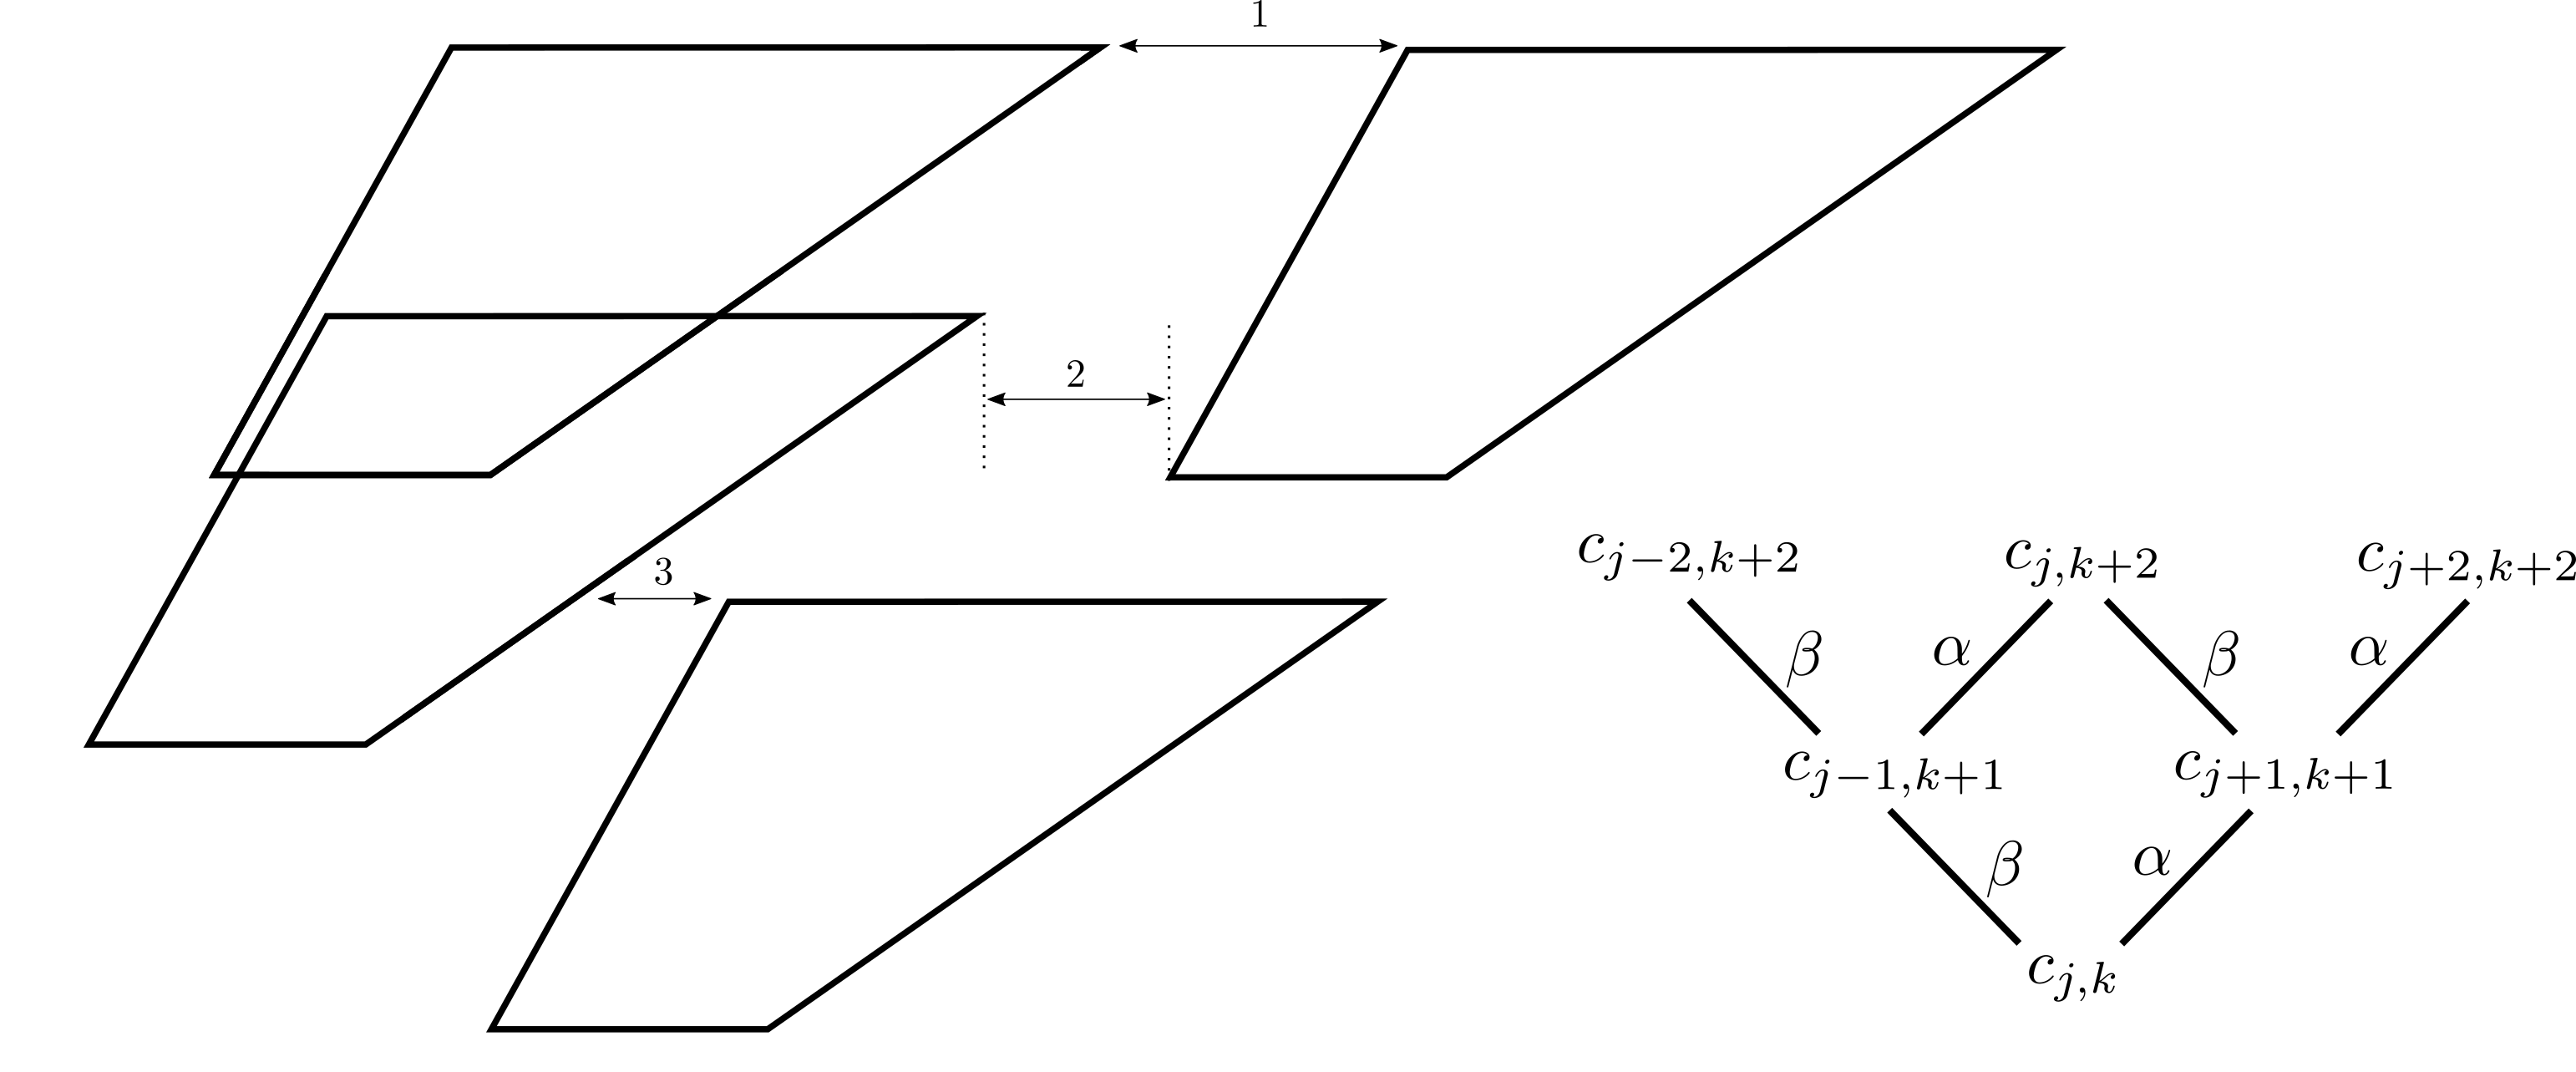
\includegraphics[width=\linewidth]{images/construction_intersections}
  \caption{The three different distances that we show are positive in the proof of Lemma \ref{lem:dependency}. }
  \label{fig:construction_intersections}
\end{figure}
\begin{lemma}\label{lem:dependency}
Independent of $L$ we can take $\delta$ small enough such that two quadrilaterals $S_{j_1,k_1}, S_{j_2, k_2}$ intersect only if $(j_1, k_1), (j_2, k_2)$ are nearest neighbours in $U$. 
\end{lemma}

\begin{proof}
Notice that both space and time are scaled by $L$ so that we may set $L = 1$ without loss of generality. Take $(j,k) \in U$. Recall that we asserted $t_m = \frac{3\delta}{\alpha - \beta} < 1$ so that quadrilaterals two or more rows apart cannot intersect. Thus it is sufficient to show that $S_{j, k} \cap S_{j - 4, k} = S_{j,k} \cap S_{j + 3, k + 1} = S_{j,k} \cap S_{j - 3, k + 1} = \varnothing$ for small enough $\delta$. For a visualisation see Figure \ref{fig:construction_intersections}. Note that the space-coordinate of $c_{j,k}$ satisfies the recursive equations

\begin{equation}\nonumber
c^{(1)}_{j,k} = c^{(1)}_{j - 1, k - 1} + \alpha L + \cal{O}(\delta L) = c^{(1)}_{j + 1, k - 1} + \beta L + \cal{O}(\delta L). 
\end{equation}
The claims follow by comparing the space-coordinate of different quadrilaterals using the above formula. 
\begin{enumerate}
\item \underline{$S_{j, k} \cap S_{j - 4, k} = \varnothing$}
\begin{flalign*}
& (\text{top left of } S_{j, k})_{space} - (\text{top right of } S_{j - 4, k})_{space} &\\
& \qquad = 2 \alpha + \beta - (2 \beta + \alpha) + \cal{O}(\delta) = \alpha - \beta + \cal{O}(\delta) &
\end{flalign*}
\item \underline{$S_{j,k} \cap S_{j + 3, k + 1} = \varnothing$}
\begin{flalign*}
& (\text{bottom left of } S_{j + 3, k + 1})_{space} - (\text{top right of } S_{j, k})_{space} &\\
& \qquad =  2 \alpha  - (\beta + \alpha) + \cal{O}(\delta) = \alpha - \beta + \cal{O}(\delta)
\end{flalign*}
\item \underline{$S_{j,k} \cap S_{j - 3, k + 1} = \varnothing$}
\begin{flalign*}
& (\text{top left of } S_{j, k})_{space} - (\text{time $t_m$ along right edge of } S_{j - 3, k + 1})_{space} &\\
& \qquad =  \alpha + \beta  - (2 \beta + \alpha t_m) + \cal{O}(\delta) = \alpha (1 - t_m) - \beta + \cal{O}(\delta) &\\
& \qquad = \alpha - \beta + \cal{O}(\delta)
\end{flalign*}
\end{enumerate}
\end{proof}

\begin{proof}[Proof of Theorem \ref{thm:percolation}]
\begin{figure}[!h]
  \includegraphics[width=\linewidth]{images/construction_tiling}
  \caption{A segment of the tiling with a single tile at $c_{j, k}$ outlined in bold. The red path shows how propagation to infinity occurs. }
  \label{fig:construction_tiling}
\end{figure}
By Lemma \ref{lem:dependency} take $\delta$ small enough such that $\{S_{j,k}\}_{(j,k) \in U}$ intersect only if they are nearest neighbours. From the graphical representation it is immediate that $E_{j,k}$ is measurable with respect to the information in $S_{j,k} \subset \scr{P}$, hence the events $\{E_{j,k}\}_{(j,k) \in U}$ are dependent only if they are nearest neighbours in $U$ i.e. the percolation model is one-dependent as required. Now, by Lemma \ref{lem:construction} as $L$ goes to infinity the density $\Pr{E}$ goes to $1$. 
\end{proof}
\begin{remark}
It is important to note that by the properties of the construction \newline $\{\text{percolation from $(0,0)$ in $\{\mathbbm{1}_{E_{j,k}}\}_{(j,k) \in U}$}\} \subset \left\{ \tau\left(\eta^{[- \frac{3 \delta L}{2}, \frac{3 \delta L}{2}]}_\cdot \right) = \infty \right\}$. To see this consider the red path on Figure \ref{fig:construction_tiling}. 
\end{remark}

\subsection{Exponential bounds}

To prove Theorem \ref{main_thm:exponential_bounds} we need a result for oriented one-dependent percolation with large density. For $n \in \N$ define 
\begin{align*}
r_n &\defeq \max\{j \mid \text{ there is an active path from $(m,0)$ to $(j,n)$ for some $m\leq 0$} \\ \nonumber&\qquad\qquad\qquad \text{in the oriented percolation model given by $\{\mathbbm{1}_{E_{j,k}}\}_{(j,k) \in U}$ }\}, 
\end{align*}
with $\max \varnothing = - \infty$. 

\begin{lemma}[{{\cite[Section 6, Theorem 3.21]{liggett2012interacting}}}]\label{lem:discrete_front}
Suppose $q < 1$. For an oriented one-dependent percolation model with density $\rho > 1 - 3^{-\sfrac{72}{(1 - q)}}$, 
\begin{equation}\nonumber
\Pr{r_n < n q} \leq 3^{-n + 1}
\end{equation}
\end{lemma}

\begin{proof}[Proof of Theorem \ref{main_thm:exponential_bounds}]
Take $\delta < \frac{\alpha - \beta}{3}$ such that it satisfies Lemma \ref{lem:discrete_front} so that $\{\mathbbm{1}_{E_{j,k}}\}_{(j,k) \in U}$ is one-dependent and take $L$ large enough such that its density satisfies Lemma \ref{lem:discrete_front}. For $t \in [nL, (n + 1)L]$ we have
\begin{equation}\nonumber
r^{(-\infty, 0]}_t \geq (\text{bottom left of $S_{r_n,n}$})_{space} = c^{(1)}_{r_n, n} - \frac{3 \delta L}{2}.  
\end{equation}
This follows after considering Theorem \ref{thm:percolation} and the remark after as well as the definition of $r_n$ and $c^{(1)}_{r_n, n}$. More precisely, there exists a path from $(-\infty, 0] \times \{0\}$ through $(c^{(1)}_{r_n, n} - \frac{\delta L}{2}, c^{(1)}_{r_n, n} + \frac{\delta L}{2}) \times \{nL\}$ up to time $\{nL + t_m\}$; furthermore since we're on $E_{r_n, n}$, we can concatenate this path with one that continues inside $S_{r_n, n}$ up until time $(n + 1)L + t_m$. This path in turn can be used to bound the right edge process from the left in the time interval $[nL, (n+1)L + t_m]$. Therefore we get
\begin{align*}
\Pr{r^{(-\infty, 0]}_t < at} &\leq \Pr{c^{(1)}_{r_n, n} - \frac{3 \delta L}{2} < a(n + 1)L} \\
			  &= \Pr{\frac{n + r_n}{2}(\alpha - \delta) + \frac{n - r_n}{2}(\beta + \delta) - \frac{3 \delta}{2} < a(n + 1)} \\
			  &= \P \Bigg(r_n < \underbrace{\frac{2a - (\alpha + \beta)}{\alpha - \beta - 2\delta}}_{ < 1 \text{ for small enough } \delta} n + \cal{O}(\delta) \Bigg), 
\end{align*}
where the order $\delta$ term is independent of $n$. It follows that for small enough $\delta$ and all large enough $n$, if $t \in [nL, (n+1)L]$ then
\begin{equation}\nonumber
\Pr{r^{(-\infty, 0]}_t < at} \leq 3^{-n + 1}, 
\end{equation}
which concludes the proof of part $(i)$. Note that analogously one can prove that for all $b > \beta$ there exist constants $\gamma, C > 0$ such that for all $t \geq 0$ we have
\begin{equation}\nonumber
\Pr{l^{[0, \infty)}_t > b t} \leq C e^{-\gamma t}
\end{equation}
To prove part $(ii)$ first take $a \in \left(\sfrac{(\alpha + \beta)}{2}, \alpha \right)$. From here on $\gamma, C > 0$ denote constants that change from line to line. By part $(i)$ we know that
\begin{equation}\nonumber
\Pr{r^{(-\infty, 0]}_m < \frac{\alpha + \beta}{2} m \text{, for some integer $m \geq N$}} \leq C e^{- \gamma N}.
\end{equation}
Since $r^{(-\infty, 0]}_t$ is majorized by a Poisson process of rate $1$ we also have
\begin{equation} \nonumber
\Pr{r^{(-\infty, 0]}_t < \frac{\alpha + \beta}{2} t \text{, for some $t \in [m, m+1]$ and }r^{(-\infty, 0]}_{m + 1} > a(m+1)} \leq C e^{- \gamma m}. 
\end{equation}
Combining the previous two inequalities gives that for all $T \geq 0$, 
\begin{align*}
\Pr{r^{(-\infty, 0]}_t < \frac{\alpha + \beta}{2} t \text{, for some $t \geq T$}} &\leq C e^{- \gamma T} \\
\intertext{As we mentioned before, analogous results for the left edge process $(l^{[0, \infty)}_t)_{t \geq 0}$ can be obtained. Using these we get}
\Pr{l^{[0, \infty)}_t \leq \frac{\alpha + \beta}{2} t \leq r^{(-\infty, 0]}_t \text{, for all $t \geq T$}} &\geq 1 - 2\, C e^{- \gamma T}. \\
\end{align*}
On the event $\{\tau(\eta^{\{0\}}_.) > T\}$ it is easy to see that $\tau(\eta^{\{0\}}_.) = \inf\{ t \geq T \mid l^{[0, \infty)}_t > r^{(- \infty, 0]}_t \}$ so that
\begin{align*}
\PrCond{\tau(\eta^{\{0\}}_.) = \infty}{\tau(\eta^{\{0\}}_.) > T} &\geq \Pr{l^{[0, \infty)}_t \leq \frac{\alpha + \beta}{2} t \leq r^{(-\infty, 0]}_t \text{, for all $t \geq T$}} \\
&\geq 1 - 2\, C e^{- \gamma T}. 
\end{align*}
The conclusion follows. 
\end{proof}

\begin{corollary}\label{cor:durrett}
If $(\eta_t)_{t \geq 0}$ is a supercritical, one-sided contact process then for all $a < \alpha$ there exist constants $\gamma, C > 0$ satisfying 
\begin{align*}\label{eqn:durret_decay}
  \PrCond{r^{\{0\}}_t < a t}{\tau(\eta^{\{0\}}_\cdot) = \infty} &\leq C e^{-\gamma t}  && \forall t \geq 0. 
\end{align*}
\end{corollary}

\begin{proof}
Note that on $\{\tau(\eta^{\{0\}}_\cdot) = \infty \}$ it holds that $r^{\{0\}}_t = r^{(-\infty, 0]}_t$ for all $t \geq 0$. 
\end{proof}

\section{Front propagation --- Proof of Theorem $2$}

\begin{quote}
{\small We prove linear speed for the front of the East model. The upper bound follows from classical results for Poisson point processes, while the lower bound is established by a comparison with the one-sided contact process, closely following the arguments of \cite{blondel2018front}. }
\end{quote}

\subsection{Restart argument}

\begin{theorem}\label{thm:restart_coupling}
For each $p < 1$ with $\frac{p}{1-p} > \lambda_c$ there exists a process $(\sigma_t, \eta_t)_{t \geq 0}$ taking values in $\Omega^2$ and a random variable $T$ taking values in $[0, \infty)$ such that 
\begin{enumerate}[(i)]
  \item $(\sigma_t)$ is a (supercritical) East model with rate parameter $p$ started from $\{0\}$
  \item $\forall t \geq 0$ and $\forall x \in \Z$, it holds that $\eta_t(x) \leq \sigma_t(x)$
  \item $(\eta_{T+t})_{t \geq 0}$ is a surviving one-sided contact process started from $\{0\}$
\end{enumerate}
Furthermore $T$ has exponentially decaying tail probabilities. 
\end{theorem}

\begin{proof}
Let $\{ \scr{C}^{(i)}\}_{i \in \N^+}$ be independent copies of $\scr{C}$. Denote by $\eta^{(i)}_.$ the one-sided contact process started from $\{0\}$, constructed using $\scr{C}^{(i)}$. Furthermore let $U_i \defeq \tau(\eta^{(i)}_.)$ be the extinction time of $\eta^{(i)}_.$. Note that the $U_i$ are i.i.d. and $\mu \defeq \Pr{U_1 = \infty} > 0$ by supercriticality. Define $L \defeq \min \{ i: U_i = \infty \}$ and note that $L$ has geometric distribution. Finally, let 
\[
T \defeq 
\left\{
  \begin{array}{ll}
    0                           & \mbox{if } L = 1 \\
    \sum\limits^{L-1}_{i=1} U_i & \mbox{otherwise}
  \end{array}
\right..
\]
First we show that $T$ has exponentially decaying tail probabilities. Note that since $T \geq 0$ almost surely, this is equivalent to finiteness of $\Ex{e^{s T}}$ for some $s > 0$. To see the latter holds for $T$ observe that conditional on $L$ the random variables $U_1, ..., U_{L-1}$ are i.i.d. with distribution equal to that of $U_1$ given $U_1 < \infty$. From Corollary \ref{cor:durrett} it follows that $U_1 | \{U_1 < \infty \}$ has exponentially decaying tail probabilities:
\begin{align*}
\Pr{U_1 > t\ | U_1 < \infty} = \frac{\Pr{t < U_1 < \infty}}{\Pr{U_1 < \infty}} \leq \frac{C e^{- \gamma t}}{1 - \mu}
\end{align*}
Therefore there exists $s > 0$ such that $\ExCond{e^{sU_1}}{U_1 < \infty} < \infty$, and so
\begin{align*}
\Ex{e^{sT}} &= \Ex{\ExCond{\exp\left(s\sum\limits_{i=1}^{L-1} U_i \right)}{L}} \\
            &= \Ex{\ExCond{e^{s U_1}}{U_1 < \infty}^{L-1}} < \infty \,,
\end{align*}
where finiteseness follows as $L$ has geometric distribution and so finite moment generating function for all $s \in \R$. \\
Now we construct the process $(\sigma_t, \eta_t)_{t \geq 0}$:
\begin{enumerate}
  \item Let $(\sigma^{[1]}_t, \eta^{[1]}_t)_{t \geq 0}$ be the basic coupling started from (\{0\}, \{0\}), constructed using $\scr{C}^{(1)}$. 
  \item Assuming $(\sigma^{[i]}_t, \eta^{[i]}_t)_{t \geq 0}$ has been constructed, define $(\sigma^{[i+1]}_t, \eta^{[i+1]}_t)_{t \geq 0}$ as :
  \begin{itemize}
    \item If $T_i \defeq \sum\limits^i_{j=1} U_j = \infty$ then $(\sigma^{[i+1]}_t, \eta^{[i+1]}_t)_{t \geq 0} \defeq (\sigma^{[i]}_t, \eta^{[i]}_t)_{t \geq 0}$
    \item Else, set $(\sigma^{[i+1]}_t, \eta^{[i+1]}_t)_{T_i > t \geq 0} \defeq (\sigma^{[i]}_t, \eta^{[i]}_t)_{T_i > t \geq 0}$ and let $(\sigma^{[i+1]}_t, \eta^{[i+1]}_t)_{t \geq T_i}$ be the basic coupling started from $(\sigma^{[i]}_{T_i}, \{0\})$, constructed using $\scr{C}^{(i+1)}$. 
  \end{itemize}
\end{enumerate}
Since $L$ has a geometric distribution, $L < \infty$ a.s. and we may define $(\sigma_t, \eta_t)_{t \geq 0} \defeq (\sigma^{[L]}_t, \eta^{[L]}_t)_{t \geq 0}$. As the $U_i$ are stopping times, $(\sigma_t)_{t \geq 0}$ is an East model started from \{0\}. It also follows that $(\eta_{T+t})_{t \geq 0}$ is a surviving one-sided contact process started from \{0\}. Noting that an East model started from \{0\} alwas has a 1 at the origin, it follows that $\eta_t \leq \sigma_t\ \forall t \geq 0$. 
\end{proof}

\subsection{Linear lower bound on propagation}

\begin{remark}
In the following proof the values of the constants $\gamma\ \&\ C$ change from line to line, without explicit mention. 
\end{remark}

\begin{proof}[Proof of lower bound in Theorem \ref{main_thm:speed}]
Let $(\sigma_t)_{t \geq 0},\ (\eta_t)_{t \geq 0}$ and $T$ be as in Theorem \ref{thm:restart_coupling}. Since $\eta_{T + .}$ survives, by Corollary \ref{cor:durrett} $\exists\ \alpha > 0$ such that for all $a < \alpha$ there exist $\gamma, C > 0$ satisfying 
\begin{align}\label{eqn:surviving_exp_decay}
  \Pr{X(\eta_{T+t}) < at} &\leq C e^{- \gamma t}  &&\forall t \geq 0. 
\end{align}
By Theorem \ref{thm:restart_coupling} part (ii) we know that $\eta_t \leq \sigma_t$ for all $t \geq 0$, so that for $c \in (0,1)$ we have
\begin{align*}
  \Pr{X(\sigma_t) < at,\ 0 \leq T \leq ct} &\leq \Pr{X(\eta_t) < at,\ (1-c)t \leq t-T \leq t} \\
                                           &=    \Pr{X(\eta_{T + (t - T)}) < at,\ t \leq \frac{t-T}{1-c} \leq \frac{t}{1-c}} \\
                                           &\leq \Pr{X(\eta_{T + (t - T)}) < \frac{a(t - T)}{1-c},\ t \leq \frac{t-T}{1-c} \leq \frac{t}{1-c}} \\
                                           &\leq \sup\limits_{u \in [(1-c)t,t]} \Pr{X(\eta_{T + u}) < \frac{au}{1-c}}. \\
  \intertext{For $c$ small enough such that $\frac{a}{1-c} < \alpha$ it follows by (\ref{eqn:surviving_exp_decay}) that}
  \sup\limits_{u \in [(1-c)t,t]} \Pr{X(\eta_{T + u}) < \frac{au}{1-c}} &\leq \sup\limits_{u \in [(1-c)t,t]} C e^{-\gamma u}  = C e^{-\gamma (1-c) t} \\
                                                                       &= C e^{-\gamma t}. \\ 
  \intertext{To get the conclusion observe that}
    \Pr{X(\sigma_t) < at}  &\leq \Pr{X(\sigma_t) < at,\ 0 \leq T \leq ct} + \Pr{T > ct} \\
                           &\leq C_1 e^{-\gamma_1 t} + C_2 e^{-\gamma_2 t} \leq C e^{-\gamma t}. 
\end{align*}
\end{proof}

\subsection{Finite speed of propagation}

\begin{definition}\label{def:hitting_times}
For the East model $(\sigma^{\{0\}}_t)_{t \geq 0}$ define $\rho_l \defeq \min\{ t \geq 0 \mid \sigma^{\{0\}}_t(l) = 1\}$ for each $l \in \N$ to be the first time that the front reaches site $l$. 
\end{definition}

Note that $0 = \rho_0 \leq \rho_1 \leq \rho_2 \leq \rho_l < \infty$ for all $l \in \N$ with finiteness following from at least linear propagation of the front since $\Pr{\rho_l = \infty} = \lim_{t \rightarrow \infty} \Pr{\rho_l > t} \leq \lim_{t \rightarrow \infty} \Pr{X\left( \sigma_t\right) < l} = 0$. We wish to bound the quantity $\Pr{\rho_l \leq t}$ to control the speed of the front since  $\{X \left( \sigma_t \right) \geq l \} \subset \{\rho_l \leq t \}$. \\

Consider the stopping times $\tau_x$ for each site $x \in \N$ defined as $\tau_{x+1} \defeq \min\{ T_{x+1, k} \mid T_{x+1, k} > \tau_x\ \text{ and } k \in \N^+ \}$ with $\tau_0 = 0$. Define the process $M_t \defeq |\{x \geq 1 \mid \tau_x \leq t \}|$ to be the process counting the number of $\tau_x$ that have occured up to time t. By repeated application of the strong Markov property it follows that the process $(M_t)_{t \geq 0}$ is in fact a Poisson process of rate 1. Define $F(M, t)$ to be the event that there is an increasing sequence of rings starting at site 1 and ending at site $M$ in the time interval $[0, t]$. By the definition of $(M_t)_{t \geq 0}$ it follows that $\Pr{F(M, t)} = \Pr{M_t \geq M}$. This, combined with the following standard result gives us the desired upper bound. 

\begin{lemma}\label{lem:chernoff}
Let $X \sim \dPoi{\lambda}$ be a Poisson random variable with mean $\lambda > 0$. Then 
\begin{align*}
\Pr{X \geq x} &\leq \frac{e^{-\lambda}(e \lambda)^x}{x^x} &&\forall x > \lambda. 
\end{align*} 
\end{lemma}

\begin{proof}
The result follows by a Chernoff bound argument. For all $t > 0$ we have
\begin{align*}
\Pr{X \geq x} &\leq \frac{\Ex{e^{tX}}}{e^{tx}} = \exp\left( \lambda e^t - \lambda - tx \right). 
\end{align*} 
The minimum occurs at $t = \log\left( \frac{x}{\lambda} \right)$, giving the result. 
\end{proof}

We are now ready to prove the linear upper bound on the speed of the East model.

\begin{remark}
In the following proof we omit the use of the floor function $\floor{\cdot}$ for clarity of notation, treating non-integer values as integers. It is however clear that the proof could be adapted to be precise. 
\end{remark}

\begin{proof}[Proof of upper bound in Theorem \ref{main_thm:speed}]
Let $v > 1$. Using Lemma \ref{lem:chernoff} and the discussion before it the calculation of an upper bound becomes straightforward:
\begin{align*}
\Pr{X(\sigma_t) > vt} &\leq \Pr{\rho_{vt} \leq t} = \Pr{M_t \geq vt} \\
                      &\leq \frac{e^{-t}(e t)^{vt}}{(vt)^{vt}} = \exp\left( -t + vt(\log\left(\sfrac{t}{vt}\right) + 1)\right) \\
                      &= \exp\left( -t + vt (1 - \log(v))\right) \leq \exp(vt (1 - \log(v)))
\end{align*}
To conclude take $v > e$ and $\gamma = - v (1 - \log(v))$. 
\end{proof}






\section{Mixing --- Proof of Theorem $3$}
\begin{quote}
{\small We prove that the mixing time of the supercritical East process on $[0, L]$ with a 1 fixed at the origin is $\Theta(L)$. }
\end{quote}

In this section we will study the evolution of the East process restricted to the segment [0, L] where $L \in \N$. In doing so we will assume that there is a 1 fixed at the origin. However, because of the local constraint of the East process, when studying the East process restricted to $\{0, 1, ..., L\}$ it doesn't matter whether we 1) fix a 1 at the origin or 2) only consider East processes started from $\{0\} \subseteq \xi \subseteq \N$; the results of the analysis will be the same. Motivated by this we make two definitions:

\begin{definition}
Define $\widetilde{\Omega} \defeq \{A \subseteq \N \mid 0 \in A \}$ to be the set of configurations that are 0 on the negatives and 1 at the origin. Similarly, for $L \in \N$ define $\Omega_L \defeq \{ A \cap [0, L] \mid A \in \widetilde{\Omega} \}$ to be the state space of the East process on $\{0, 1, ..., L\}$ with a fixed 1 at the origin. 
\end{definition}

Another important property of the East process is that the evolution at some site $x \in \N$ is not influenced by how the process evolves at sites to the right of $x$. More precisely, if $(\sigma_t)_{t \geq 0}$ is an East process then for any $x \in \N$ and $t \geq 0$, $\sigma_t (x)$ is independent of the sigma algebra $\sigma \left( (E_{n,k}, B_{n,k})_{n > x, k > 0}\right)$. Furthermore, if we fix a 1 at the origin (or equivalently start from a configuration in $\widetilde{\Omega}$) then an even stronger independence holds in that the evolution to the right of the origin is independent of all the clock rings and coin tosses left of the origin. Therefore the East process with a fixed 1 at the origin is a continuous time Markov chain when restricted to $\{0, 1, ..., L\}$. 

\subsection{Coupling time}
As before, let $(\sigma^\xi_t)_{t \geq 0}$ denote the East process on $\Z$ started from initial configuration $\xi \in \Omega$, constructed using $\scr{C} = (E_{x,k}, B_{x,k})_{x \in \Z,\ k \in \N^+}$. Recall the definition of the hitting times $(\rho_i)_{i \in \N}$ from Definition \ref{def:hitting_times}.  


\begin{proposition}\label{prop:East_linear_coupling}
For each $l \in \N$ and for all $\xi, \nu \in \widetilde{\Omega}$ it holds that 
\begin{align*}
\sigma^\xi_{\rho_l + t} \cap [0, l] &= \sigma^\nu_{\rho_l + t} \cap [0, l] &&\forall t \geq 0. \label{eqn:hitting_coupling}
\end{align*}
\end{proposition}

\begin{proof}
We only prove (\ref{eqn:hitting_coupling}) for $\nu = \{0\}$ from which the result follows easily for arbitrary $\nu$. We proceed by induction. The claim clearly holds for $l=0$ since every such $\xi$ has a 1 at the origin forever. For the induction step suppose that the claim holds up to $l=n \geq 0$. If $K$ is such that $T_{n+1, K} = \rho_{n+1}$ then $B_{n+1, K}=1$, and since the ring is legal, $\sigma^{\{0\}}_{\rho_{n+1}}(n) = 1$. By the induction hypothesis also $\sigma^\xi_{\rho_{n+1}}(n) = 1$ i.e. the ring is also legal for $\sigma^\xi_.$. Thus both processes update to 1 at time $\rho_{n+1}$. Now, since the $\rho_i$ are stopping times, $(\sigma^{\{0\}}_{\rho_{n+1}+t})_{t \geq 0}$ and $(\sigma^\xi_{\rho_{n+1} + t})_{t \geq 0}$ are two East processes with $\sigma^{\{0\}}_{\rho_{n+1}} \cap [0, n+1] = \sigma^\xi_{\rho_{n+1}} \cap [0, n+1] $. The conclusion follows by basic coupling. 
\end{proof}

We present a standard result for continuous time Markov chains that combined with the previous proposition gives us a powerful tool. 

\begin{theorem}\label{thm:equilibrium_distance}
Let $N \defeq (N_t)_{t \geq 0}$ be a continuous time, irreducible Markov chain taking values in a finite state space $\Omega$ and let $\pi$ be its equilibrium distribution. Suppose that for each pair of states $x,y \in \Omega$ there is a coupling $(X_t, Y_t)_{t \geq 0}$ of $N$ that is started from $(x,y) \in \Omega^2$. For each of these couplings, let $\tau^{x, y}_{couple} \defeq \min\left\{t \geq 0 \mid X_t = Y_t \right\}$ be the first time the chains meet. Then it holds that 
\begin{equation}\nonumber
d(t) \leq \max\limits_{x,y \in \Omega} \Pr{\tau^{x, y}_{couple} > t}
\end{equation}
\end{theorem}

\begin{proof}
The result can be found in \cite[Corollary 5.3]{levin2017markov} for discrete time Markov chains, however all the necessary proofs work in the continuous time case without modification. 
\end{proof}

\subsection{Linear upper bound on mixing}

\begin{proof}[Proof of upper bound in Theorem \ref{main_thm:mixing}]
By Theorem \ref{thm:equilibrium_distance} it holds that 
\begin{equation}\nonumber
d(t) \leq \max\limits_{\nu, \xi \in \widetilde{\Omega}} \Pr{ \tau^{\nu, \xi}_{couple} > t }
\end{equation}
Where $\tau^{\nu, \xi}_{couple}$ is the first time that the East process started from $\xi$ and $\nu$ (and thus with a fixed 1 at the origin) coincide on $\{0, 1 ... L\}$ under the basic coupling. Lemma \ref{prop:East_linear_coupling} gives $\max\limits_{\nu, \xi \in \widetilde{\Omega}} \Pr{\tau^{\nu, \xi}_{couple} > t } \leq \Pr{\rho_L > t}$. Take $\alpha > 0$ such that Theorem \ref{main_thm:speed} is satisfied. We have
\begin{align*}
\Pr{\rho_L > KL} &\leq \Pr{X\left(\sigma^{\{0\}}_{KL}\right) < L} \\
                 &= \Pr{X\left(\sigma^{\{0\}}_{KL}\right) < \frac{KL}{K}}. \\
  \intertext{Fix $K$ large enough such that $\sfrac{1}{K} < \alpha$ to get}
                \Pr{X\left(\sigma^{\{0\}}_{KL}\right) < \frac{KL}{K}} &\leq C e^{-\gamma K L}. 
\end{align*}
Thus there exists $L' \in \N$ such that for all $L \geq L'$ it holds that $\Pr{X\left(\sigma^{\{0\}}_{KL} \right) < L} \leq \sfrac{1}{4}$. This implies that $d(KL) \leq \sfrac{1}{4}$ in other words that $T^L_{mix} \leq KL$ for all $L \geq L'$. 
\end{proof}

\subsection{Linear lower bound on mixing}

\begin{proof}[Proof of lower bound in Theorem \ref{main_thm:mixing}]
From the proof of the upper bound in Theorem \ref{main_thm:speed} we know that $\exists\ \gamma, v > 0$ such that $\Pr{\rho_{tv} \leq t} \leq e^{- \gamma t}$ for all $ t \geq 0$. Thus we get for all $L \in \N$
\begin{equation}\nonumber
\Pr{\rho_{\sfrac{L}{2}} \leq \sfrac{L}{2v}} \leq e^{- \gamma \frac{L}{2v}} \\ \label{eqn:half_hit_bound}
\end{equation}
Define the set $A_L \defeq \{\omega \in \Omega \mid [\sfrac{L}{2},L] \cap \omega \neq \varnothing\}$ to be the set of configurations with at least one occupied site between $\sfrac{L}{2}$ and $L$. For our proof it is crucial to note that
\begin{equation}\nonumber
\PrCond{\sigma^{\{0\}}_t \in A_L}{\rho_{\sfrac{L}{2}} > t} = 0:
\end{equation}
since $(\sigma^{\{0\}}_t)_{t \geq 0}$ is started from $\{0\}$, it is infected at some site $x \in \N^+$ only if site $x$ has been hit by the front i.e. it can only happen on $\{ \rho_x \leq t \}$. Let $\pi_L \defeq \delta_1 \times \dBer{p}^L$ be the product Bernoulli measure on $\Omega_L$. We have
\begin{align*}
d\left(\frac{L}{2v}\right) &= \max\limits_{\xi \in \widetilde{\Omega}} \left\Vert \Pr{\sigma^\xi_{\sfrac{L}{2v}} \cap [0,L] \in \cdot} - \pi_L(\cdot)								   \right\Vert_{TV} \\
						   &= \max\limits_{\xi \in \widetilde{\Omega}} \max\limits_{A \in \Omega_L} \left| \Pr{\sigma^\xi_{\sfrac{L}{2v}} \cap [0,L] \in A} - \pi_L(A) \right|\\
						   &\geq \left| \Pr{\sigma^{\{0\}}_{\sfrac{L}{2v}} \in A_L} - \pi_L(A_L) \right| \\
						   &= \Big| \underbrace{\Pr{\rho_{\sfrac{L}{2}} \leq \sfrac{L}{2v}}}_{\in [0, e^{- \gamma \frac{L}{2v}}] \text{ by (\ref{eqn:half_hit_bound})}} \PrCond{\sigma^{\{0\}}_{\sfrac{L}{2v}} \in A_L}{\rho_{\sfrac{L}{2}} \leq \sfrac{L}{2v}}  - \left( 1 - q^{\sfrac{L}{2}} \right) \Big|. \\
\end{align*}
Letting $L$ go to infinity we obtain $d\left(\frac{L}{2v}\right) \xrightarrow{L \rightarrow \infty} 1$. Therefore there exists $L' \in \N$ such that for all $L \geq L'$ it holds that $d\left(\frac{L}{2v}\right) > \sfrac{1}{4}$, or in other words $\frac{L}{2v} < T^L_{mix}$ for all $L \geq L'$.
\end{proof}

\bibliographystyle{plain}
\bibliography{bibliography}

\end{document}